\section{Linear Independent Component Analysis} 

  PCA and factor analysis have found an enormous number of applications. In fact, it is one of the go-to methods for EDA, and exploratory factor analysis (EFA) is often synonymous with PCA. 

  However, a shortcoming of FA is that we can't even identify factor directions since the loading matrix $W$ can be rotated to produce just as good of a model. Therefore, Pierre Comon in 1992 had produced \textit{independent component analysis} (ICA). It is essentially a method to separate a multivariate signal into additive, statistically independent components. It does come with a lot of assumptions, and is a specific instance of a linear factor model where $\mu = 0$ and $\epsilon = 0$. 

  \begin{definition}[Linear ICA]
    In \textbf{linear ICA}, we model the true distribution of $x$ as 
    \begin{equation}
      x = W z, \qquad z \sim \mathbb{P}_z
    \end{equation}
    where $x$---the \textbf{mixture vector}---and $z$ are random variables of $\mathbb{R}^d$ and $\mathbb{R}^k$, and $W \in \mathbb{R}^{d \times k}$ is a \textbf{mixing matrix}. The parameters are both $W$ and $z$, and we need to recover them given $x$. We have 2 strong assumptions. 
    \begin{enumerate} 
      \item Each component of $z$ is independent (not just uncorrelated). 
      \item Independent components of $z$ must \textit{not} be Gaussian. This is needed for us to be able to ``unmix'' the signals.\footnote{ To see why, just suppose $z$ was Gaussian, and so the vector $Rz$ is also Gaussian for any invertible $R$. Therefore, we could find an infinite number of solutions of form $x = W R^{-1} R z$ and have no way to separate them.}
    \end{enumerate}
  \end{definition}

  \begin{algo}[Fitting]
    Now let's see how linear ICA actually estimates $W$ and $z$. Once $W$ is estimated, the latent components of a given test mixture vector, $x^\ast$ is computed by $z^\ast = W^{-1} x^\ast$. So now all there's left to do is to estimate $W$, which we want to estimate so that $W^{-1} x$ is far from Gaussian. The reason for this is that given a bunch of independent non-Gaussian $h_i$'s, if we mix them with a matrix that is not $\pm I$ , then by CLT, a linear combination of random variables will tend to be Gaussian, and so for an arbitrary $W$ we would expect $x$ to be Gaussian. Therefore, what we want to do is guess some matrix $A$, and compute 
    \begin{equation}
      A x = A W h
    \end{equation}
    and if we get things right, $A \approx W^{-1}$, and the result of $A x$ would look pretty non-Gaussian. If it it not the case, then $A W$ will still be some mixing matrix, and so $A x$ would look Gaussian. So now the question reduces to how do we choose this $A$? There are multiple ways to measure non-Gaussianity: 
    \begin{enumerate} 
      \item The absolute or squared kurtosis, which is $0$ for Gaussians. This is a differentiable function w.r.t. $W$, so we can try maximizing it. This is done for the sample kurtosis, of course.  
      \item Another measure is by maximizing the neg-entropy. 
    \end{enumerate}
  \end{algo}

  There are further ambiguities with ICA regarding uniqueness of a best representation. For one, we can only estimate the latent components up to a scaling factor since we will still get
  \begin{equation}
    x = (\alpha W) (\frac{1}{\alpha} z) \text{ for some } \alpha > 0
  \end{equation}
  We can fix this by forcing $\mathbb{E}[z_i^2] = 1$. However, there is still an ambiguity for the sign of hidden components, but this is insignificant in most applications. Second, we can estimating the components up to permutation. We have 
  \begin{equation}
    x = W P^{-1} P z
  \end{equation}
  for some permutation matrix $P$. 

  \begin{example}[Blind Source Separation]
    The canonical example of ICA is \textit{blind source separation}. 
    \begin{figure}[H]
      \centering 
      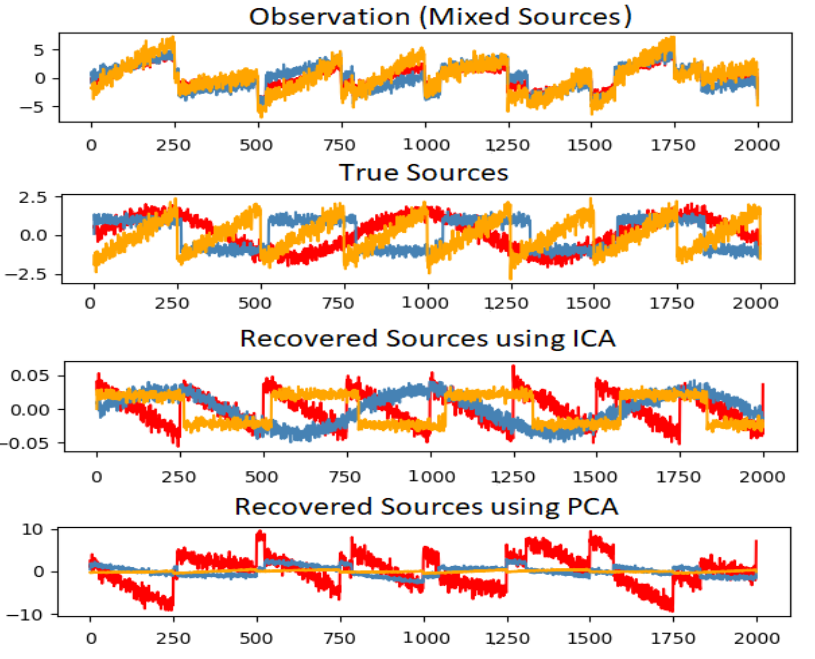
\includegraphics[scale=0.4]{img/ICA_example.png}
      \caption{We can perform this on three mixed signals with additive noise, and ICA does very well, though again some recovered signals are scaled or permuted weirdly. }
    \end{figure}
  \end{example}

